\chapter{Subsystem Design\label{chap4}}
In this chapter, we discuss the subsystem design from 5 scopes. In Section \ref{sec4.1}, the construction of environment in Webots is introduced. Then we present the visual processing in Section \ref{sec4.2}. The decision making part comes after it in Section \ref{sec4.3}, followed by the rover modeling in Section \ref{sec4.4}. The system architecture comes last in Section \ref{sec4.5}.

\section{Environment Building\label{sec4.1}}
The construction of environment is the first step of the project. Only based on a high degree of reduction environment, could the developed rover’s functions  truly meet the requirements. The construction of environment can be divided into six steps: (1) learning Webots tutorials\cite{tutorial}; (2) sorting out project requirements; (3) selecting model; (4) building model and selecting alternatives; (5) organizing component location; (6) adjusting parameters. There are two members in the Environment Group, Huiyu xiong and Jinwei Chu, who deal with requirements sorting \& components selection and model Construction \& parameters adjustment respectively.


\subsection{Requirements sorting \& Components selection}
Author: Huiyu XIONG, UoG ID: 357680X\\

As the basis of intelligent rover project, environment is a very important part. Because an untrue environment may cause some problems in the R \& D stage of the project and then affect its practical application. In the environment, any trace element may have a great impact on the project design. For example, light intensity will affect the selection of visual sensor and algorithm, etc. In this case, considering the real reduction environment and careful analysis of project requirements, it is necessary to organize and summarize the project model.

The first is to interpret the project requirements. From the TDPS Course on Moodle \ref{course_website}, we downloaded the requirements for this project and the latest supplementary requirements for the online simulation project. Combining the information of these PDF files with the supervisors' reply to the students' questions on the MS team, we sorted out the overall requirements of the environment: to build a world marked with size as shown in Figure \ref{fig:environment}, in which some patrol lines are drawn from start, so that the rover (50 cm x 50 cm) can follow. Next, there is an orange beacon or box on the edge of the pond, where fish feed. Additionally, the bridge (100cm(W) x 3m(L)), including the ramp used to get up and down the bridge, will be aligned with the edge of the pond in the middle. After crossing the bridge, several trees scattered randomly. Avoiding it, the gate (slightly larger than the rover, the recommended size is (100cm (W) x 100cm (H)) can be found by beacon. Then, go through it and follow the line on the ground. Move to the color box. After the rover reads the color of the box, the rover should be able to follow the correct color until it reaches finish.

According to this requirement, we drew out several important models to build the world: line patrol; pond \& river; bridge; gate; trees; beacons and some invisible conditions. By comparing the requirements of each node and project, we have found several suitable components. 

The first is line patrol, which is composed of four curved road segments with different radii and five straight road segments. The different curve design is to make the project more difficult, so as to verify the powerful patrol function of our rover. 

In order to build a real pond and river, we choose the fluid node. The yellow Duckling floating on the water in Figure \ref{fig:duck} reflects the buoyancy of liquid water, which shows that our environment is close to reality. One more thing to be mentioned here is that this duckling  causes no interference to the recognition  of bridge, which verifies the robustness of our visual algorithms.

\begin{figure}[htbp]
    \centering
    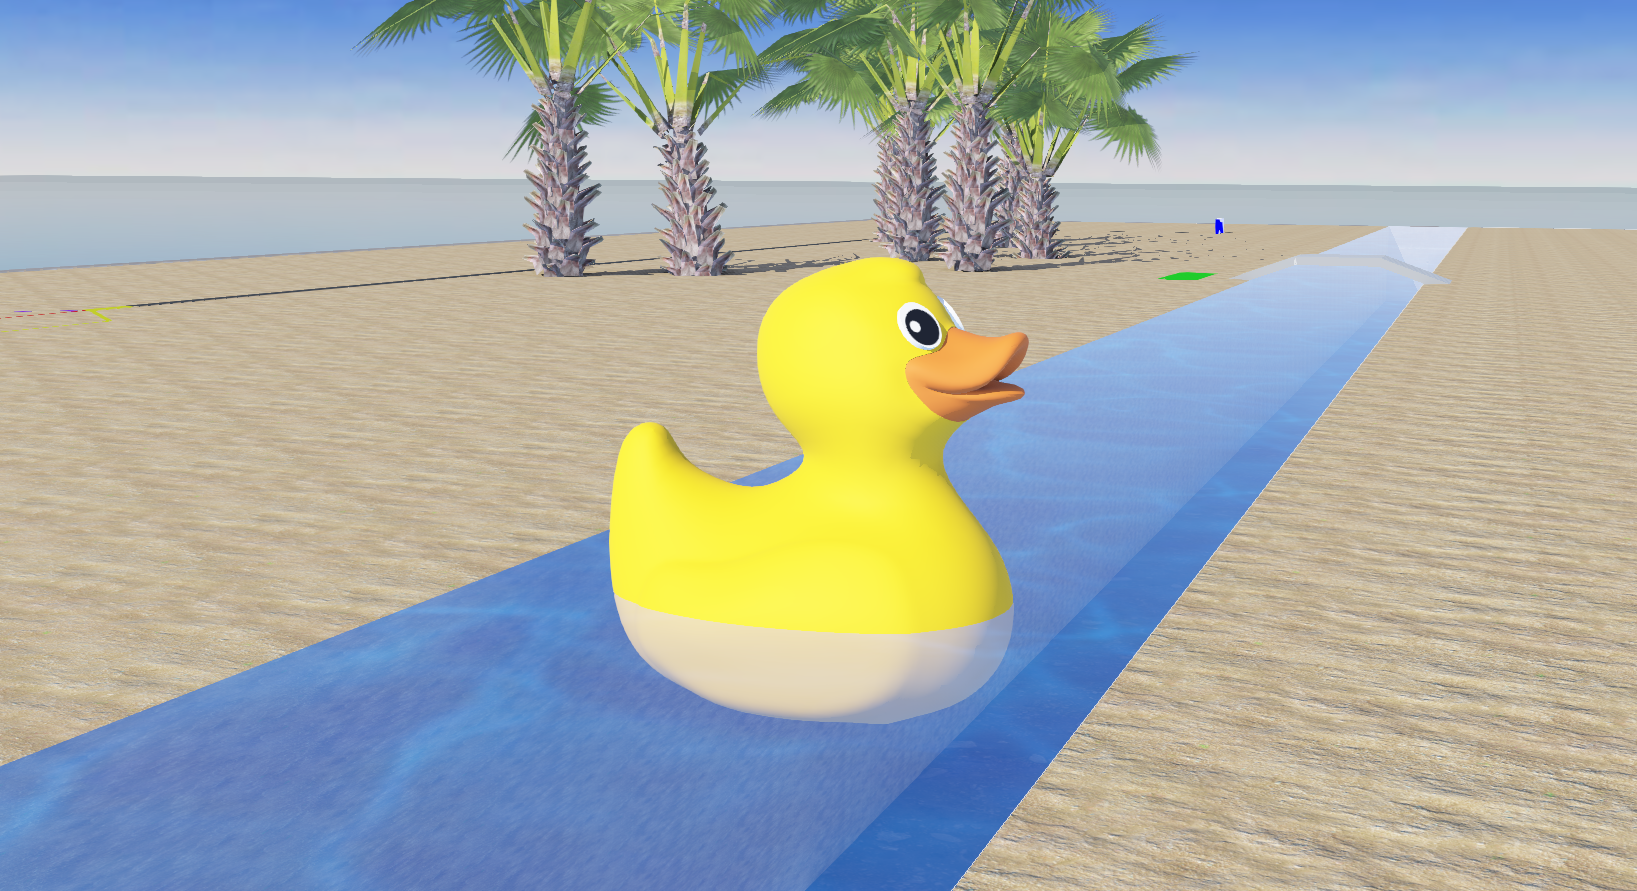
\includegraphics[width=12cm]{implementation/img_xiong/duck.png}
    \caption{The floating yellow ducking}
    \label{fig:duck}
\end{figure}

After the choice of sandy land, the choice of forest is of course the palm tree. In order to reflect the strong visual recognition ability of rover, we use the beacon as little as possible in the whole project. Color boxes are considered as beacons, which only use three places in total: Orange boxes for fish; green boxes after crossing the bridge and color boxes with undetermined colors in the final task.

\begin{figure}[htbp]
    \centering
    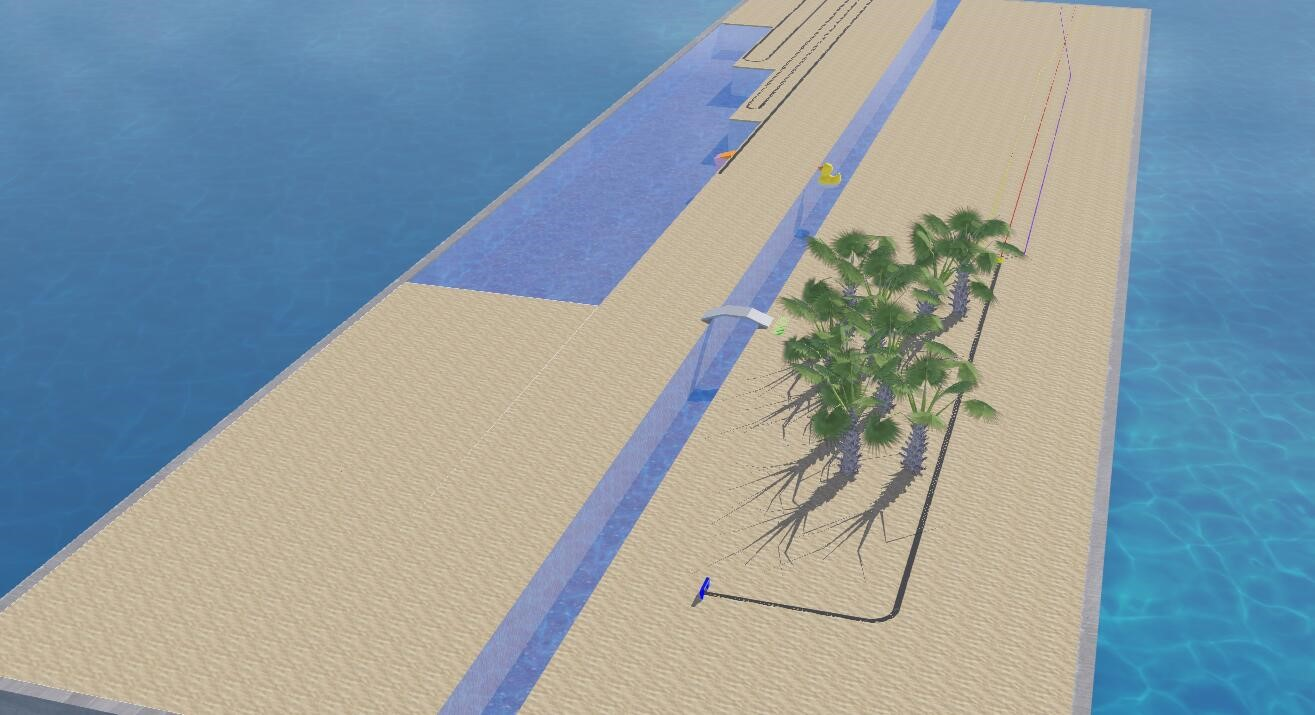
\includegraphics[width=12cm]{implementation/img_xiong/environment.jpg}
    \caption{The construction of palm trees}
    \label{fig:environment}
\end{figure}

After browsing all the nodes, we found that it is difficult to find the appropriate nodes for components with special shape and size, such as gates and bridges. The specific solutions to this part will be described in the next section written by Jinwei Chu.

Finally, it is worth mentioning some invisible conditions, such as background conditions: light, background ocean and ground. We use “noon-sunny-empty” here. In order to simulate the intensity of sunlight at noon. It is said that light intensity will affect visual judgment, so we want to consider this extreme environmental impact factor. On the periphery of the environment, we added an ocean. The world itself is covered by solid in the sand. Together, it forms a picturesque summer island.
%-----------------------------------------------------------------------
\subsection{Environment Modeling \& Parameter Adjustment}
Author: Jinwei CHU, UoG ID: 2357643C\\

The key part of the environment modeling is the construction of the bridge and the gate. After seeking for the substitution of the bridge and the gate, we found that there is not a satisfying substitution for these two articles in the repository. Finally, we decided to build our own model to import the model into Webots. Our constructed bridge and gate are shown in Figure \ref{fig:bridge_and_gate}. In order to meet the requirement of the handbook, we set the width of the bridge to one meter and the length of the bridge to three meters. In order to enhance the precision of the detection of the gate, we set the gate just as large as the size of the rover, which is about 50 centimeters high and 30 centimeters wide. 

\begin{figure}[htbp]
    \centering
    \subfigure[The bridge]{
    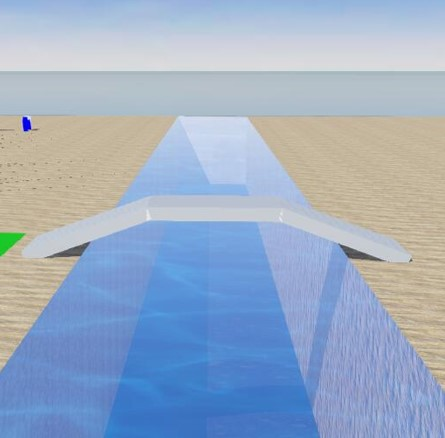
\includegraphics[width=6cm]{implementation/img_chu/bridge.jpg}
    }
    \subfigure[The gate]{
    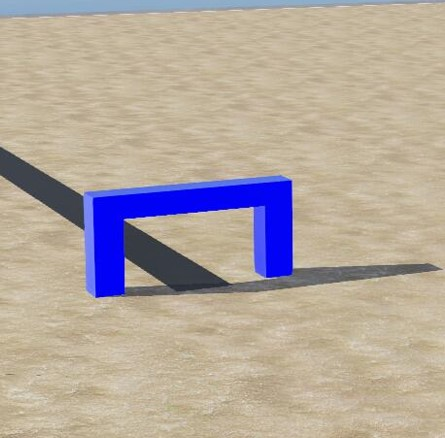
\includegraphics[width=6cm]{implementation/img_chu/gate.jpg}
    }
    \caption{The construction of the bridge and gate}
    \label{fig:bridge_and_gate}
\end{figure}

There are also some other items needed to be modeled in Webots. In task 2, the rover is expected to throw the fish food onto an orange box, where it can slide into the pond. As is shown in Figure \ref{fig:orange_box}, we put a slope onto the top of the fish box so that the fish food can be put onto the slope and then it can roll-off the slope automatically.

\begin{figure}[htbp]
    \centering
    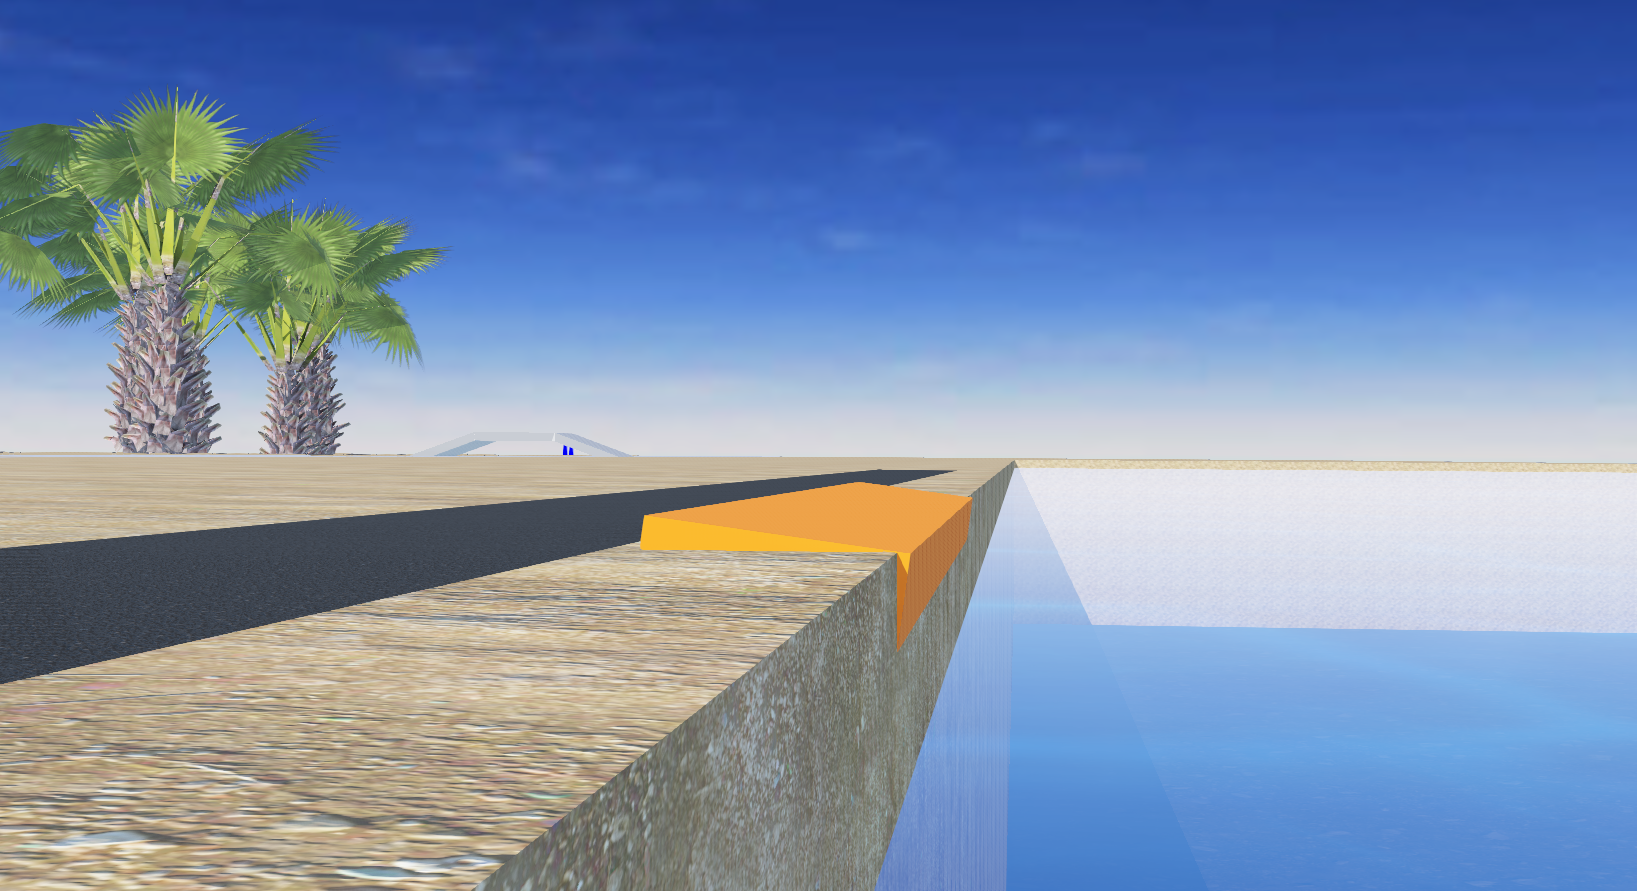
\includegraphics[width=12cm]{implementation/img_chu/orange_box.png}
    \caption{The orange box with slope}
    \label{fig:orange_box}
\end{figure}

On top of the orange box, another color box is required to be built in order to complete the Task 5. We set the color paths into three different colors: purple, yellow, and red. The width of the colorful paths is different from the width of the road, which is about 0.1 meter wide. We do this deliberately to test the robustness of our path finding algorithm. Our constructed color box and path is shown in Figure \ref{fig:color_box}.

\begin{figure}[htbp]
    \centering
    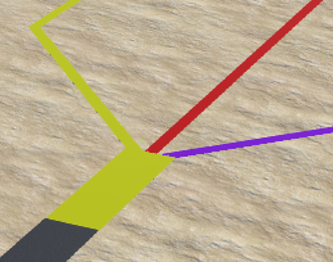
\includegraphics[width=6cm]{implementation/img_chu/color_box.png}
    \caption{The constructed color box and path in Task 5}
    \label{fig:color_box}
\end{figure}

In summary, the advantages of our design are listed below:
\begin{itemize}
    \item In order to make the environment more realistic, we converted the texture of the floor into sand, which looks just the same as the ground near the east lake of our school.
    \item In order to modify the texture of the ground, we use this several boxes to form the ground rather than use the default ground.
    \item The water used in our environment is constructed with the node fluid. In order to show its physical property, we put a rubber duck on the water, which can be seen that the rubber duck is floating on the water.
    \item In order to test the stability of our system. When we were constructing the road, at the corner of the road, we used different radius so that if the rover can turn left or turn right successfully with different radius, it shows that the stability of our system is truly good.
    \item In order to throw the fish food successfully into the pond, we put a slope on the top of the orange fish food box so that the food can be thrilled successfully into the pond.
    \item Also, in order to test the stability of power system, the gate is just as high as the height of the rover, and also the width of the gate is designed just as wide as the rover.
\end{itemize}
%-----------------------------------------------------------------------
\section{Visual Processing\label{sec4.2}}
Serving as "eyes" of the Mihotel Rover, the main work of our visual system is to perceive information from external environment and feed it to the decision module, where instructions are made to control the movement of the rover.  To ensure a robust perception of the external information, our team propose to deal with the visual processing in a gradual, goal-oriented fashion. Our goal is to choose the most suitable sensors to finish the five tasks smoothly. In particular, the rover need to find the path and detect objects such as the bridge and the gate. 

However, the selection and implementation of sensors is dependent of our solution to do the tasks, so we develop the path finding and object detection algorithms ahead of it. Before developing algorithms to do the detection, we do the image pre-processing first to obtain and remove the color information of the captured image. Three members in the Visual Group, Chang Shu, Bo Wen and Haoran Han are responsible for them respectively.
%-----------------------------------------------------------------------
\subsection{Beacon Detection \& Color Filtering\label{sec4.2.1}}
Author: Chang SHU, UoG ID: 2357702S\\

Similar to the real-world scenario, the world in Webots is riotous with color. The color is a special attribute to every item in the world and is of vital importance to our project. To be specific, the color helps us identify the fish tank and the beacon. On top of this, we also utilize color information to follow the right path in Task 5.

However, the color can sometimes be problematic. When constructing the environment in Webots, we not only set the scene, but try to make it true to life as well. Our target is to develop a robust visual system that has as good performance even in the real world. The color variation caused by the reflection of the ground, the shadow of the sunlight are taken into consideration.

\begin{figure}[htbp]
    \centering
    \subfigure[Detection of fish tank with orange box]{
    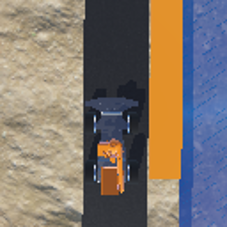
\includegraphics[width=4cm]{implementation/img_shu/beacon_orange.png}
    }
    \subfigure[Detection of turning point with green box]{
    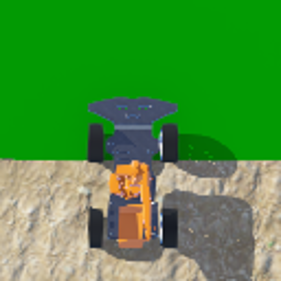
\includegraphics[width=4cm]{implementation/img_shu/beacon_green.png}
    }
    \caption{Beacon detection with color}
    \label{fig:beacon_detection}
\end{figure}

To make full use of the color information and reduce its side effects on our path finding to the least, we design a \textbf{beacon detection algorithm} and a \textbf{color filtering algorithm}. As is illustrated in Figure \ref{fig:beacon_detection}, the beacon detection algorithm looks for interested colors and returns corresponding signals when they are detected. In contrast, the color filtering does not care about the color information. It processes the unsmooth image captured by the camera and converts it into the gray image (path with black line) or binary image (path with color in Task 5) so that our path finding algorithm only needs to deal with non-color images.

The first problem to be settled is in which color space should we capture and then remove the color of images. There are some forms of color space, such as RGB (an abbreviation for Red, Green, Blue) and HSV (an abbreviation for Hue, Saturation, Value), where we can do the image processing. Although RGB is the most commonly used color space in the digital image processing, we choose to do the image processing with color in HSV space. This is because the HSV color space has the strength of separating color apart easily. 

\begin{figure}[htbp]
	\centering
	\subfigure[RGB space]{
		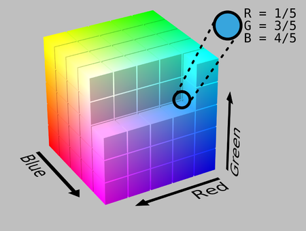
\includegraphics[width=5cm]{implementation/img_shu/rgb.png}}
	\subfigure[HSV space]{
		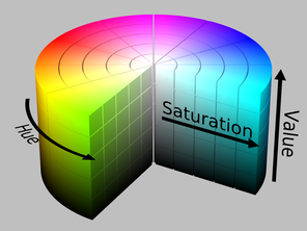
\includegraphics[width=5.07cm]{implementation/img_shu/hsv.png}}
	\caption{Illustration of two color spaces}
	\label{fig:Color Space}
\end{figure}

As is shown in Figure \ref{fig:Color Space}, the RGB color space is in the rectangular coordinate system while the HSV color space is a cylindrical-coordinate color model.  A typical color in RGB space is a weighted sum of three-primary colors, which is not intuitive. However, in the HSV space, we can find the range of each color by determining its hue first, then the saturation, and finally the value. This makes it easy for us to fix the threshold of different colors. The range of each color is found using Python GUI.

Another issue is to remove noise in the unsmooth images. As is mentioned before, the color is not a fixed value in the real-world scenrio. Even a change in the angle of sunlight may influence the range of colors. Also, the dust on the path will make it difficult for our path finding algorithm to successfully detect the path. Therefore, we propose to smooth the images with the low pass filter (LPF) and remove the noise with the opening operation. Among a wide range of LPFs, including average filter, Gaussian filter, median filter and bilateral filter, we select the Gaussian filter empirically\cite{basu2002gaussian}. The opening operation is developed from mathematical morphology, which is an erosion followed by a dilation. The erosion is used remove unwanted small pixels, like the noise in the image, while the dilation can fill the small gaps.

To mimic the reality and ensure the robustness of our visual algorithms, We manually add some Gaussian noise to our images during experiments. In Figure \ref{fig:exp1}, we convert the HSV image of roads in Task 5 into binary image with only the color box and corresponding path preserved. Unfortunately, the thresholding cannot exclude the white noise efficiently. Hence, Gaussian filter and opening operation are applied to deal with it. 

\begin{figure}[htbp]
    \centering
    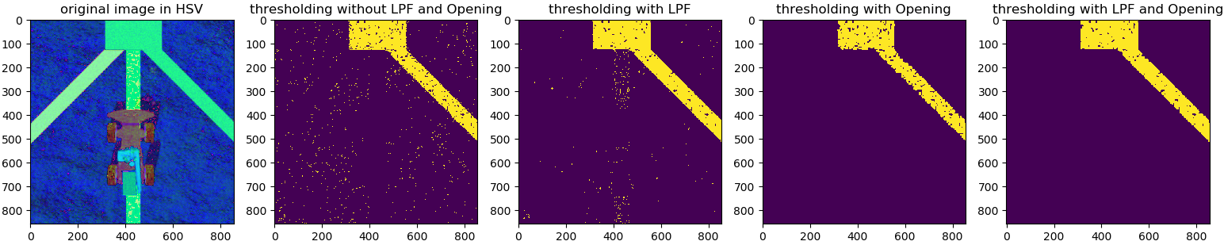
\includegraphics[width=14cm]{implementation/img_shu/experiment1.png}
    \caption{The pre-processing on the binary HSV image with 1\% Gaussian noise}
    \label{fig:exp1}
\end{figure}

As we can observe, the opening operation does a even better job than the LPF, successfully removing all the noise in the image. However, the integrity of the wanted color suffers slight loss. This problem is more significant in Figure \ref{fig:exp2}, where the color box and path directly disappears after the opening operation. This is caused by an increased amount of noise added to the image, which makes region of the wanted color discontinuous.

\begin{figure}[htbp]
    \centering
    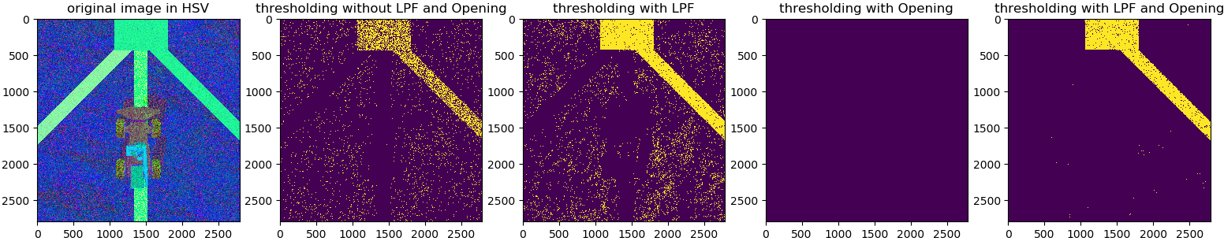
\includegraphics[width=14cm]{implementation/img_shu/experiment2.png}
    \caption{The pre-processing on the binary HSV image with 5\% Gaussian noise}
    \label{fig:exp2}
\end{figure}

The problem above is easily solved with the help of the LPF. As is discussed above, the Gaussian filter provides no better results than the opening operation. The reason is that the Gaussian filter actually works on the whole color space rather than the interested color. However, this does not mean the LPF is useless. In fact, it prevents the noise from making the region of the wanted color become discontinuous. The last image in Figure \ref{fig:exp2} shows that a combination of LPF and opening operation proves effective, both removing the noise and avoiding over-filtering.

\begin{figure}[htbp]
    \centering
    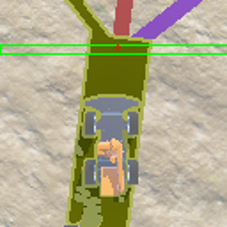
\includegraphics[width=3.5cm]{implementation/img_shu/task5_1.png}
    \caption{The principle of color path following in Task 5}
    \label{fig:task5}
\end{figure}

Finally, we are able to obtain a clear and clean binary image. To explain the principle of how we do the task 5, this is added to the original image in Figure \ref{fig:task5} as a mask. Although the input to the visual system is the RGB image, our rover is  actually following the color filtered line in the binary image.
%-----------------------------------------------------------------------
\subsection{Path Finding \& Object Detection}
Author: Bo WEN, UoG ID: 2357658W\\

As is discussed in Section \ref{sec2.1}, in Task 1 and 5, and the period between Task 4 and 5, the rover needs to detect and follow the path on the ground; In task 2,3 and 4, the rover needs to detect specific objects and react correspondingly at the correct location. We offer solutions by developing a \textbf{path finding algorithm} and a \textbf{object detection algorithm}.

\begin{figure}[htbp]
    \centering
    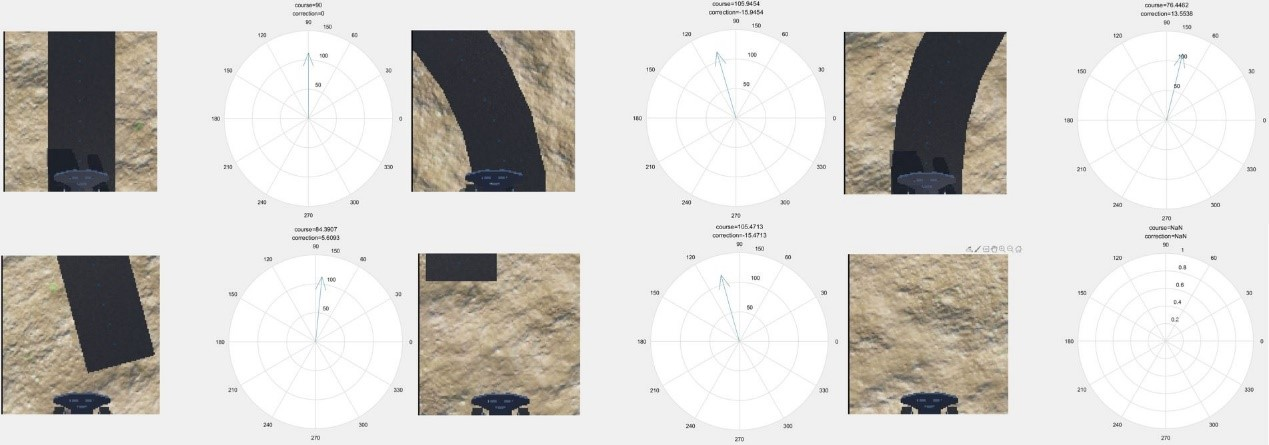
\includegraphics[width=14cm]{implementation/img_wen/path_finding.jpg}
    \caption{path finding by outputting the angle of the trajectory}
    \label{fig:path}
\end{figure}

To give an accurate and effective instruction to the rover of where it should head towards, we need to both detect the trajectory of the path and analysis the relative position of the rover to the path, then calculate an optimal correction angle for the Decision Group. With the help of the color filtering algorithm in Section \ref{sec4.2.1}, the RGB images are converted into smooth and noise-free gray (for black path) or binary (for path with color) images. Based on the grayscale feature of images to identified path pixels in the image, we vertically divide the image into several segments and calculate the geometric center of path in each segments, which form the trajectory of the path\cite{gao2012new}. Then, we determine the geometric relationship between the path and the rover by both the morphology of the path and the relative position to calculate an optimal target pixel. Consequently, our algorithm is able to give useful instructions to the rover under various of scenarios. The results are illustrated in Figure \ref{fig:path}.

\begin{figure}[htbp]
    \centering
    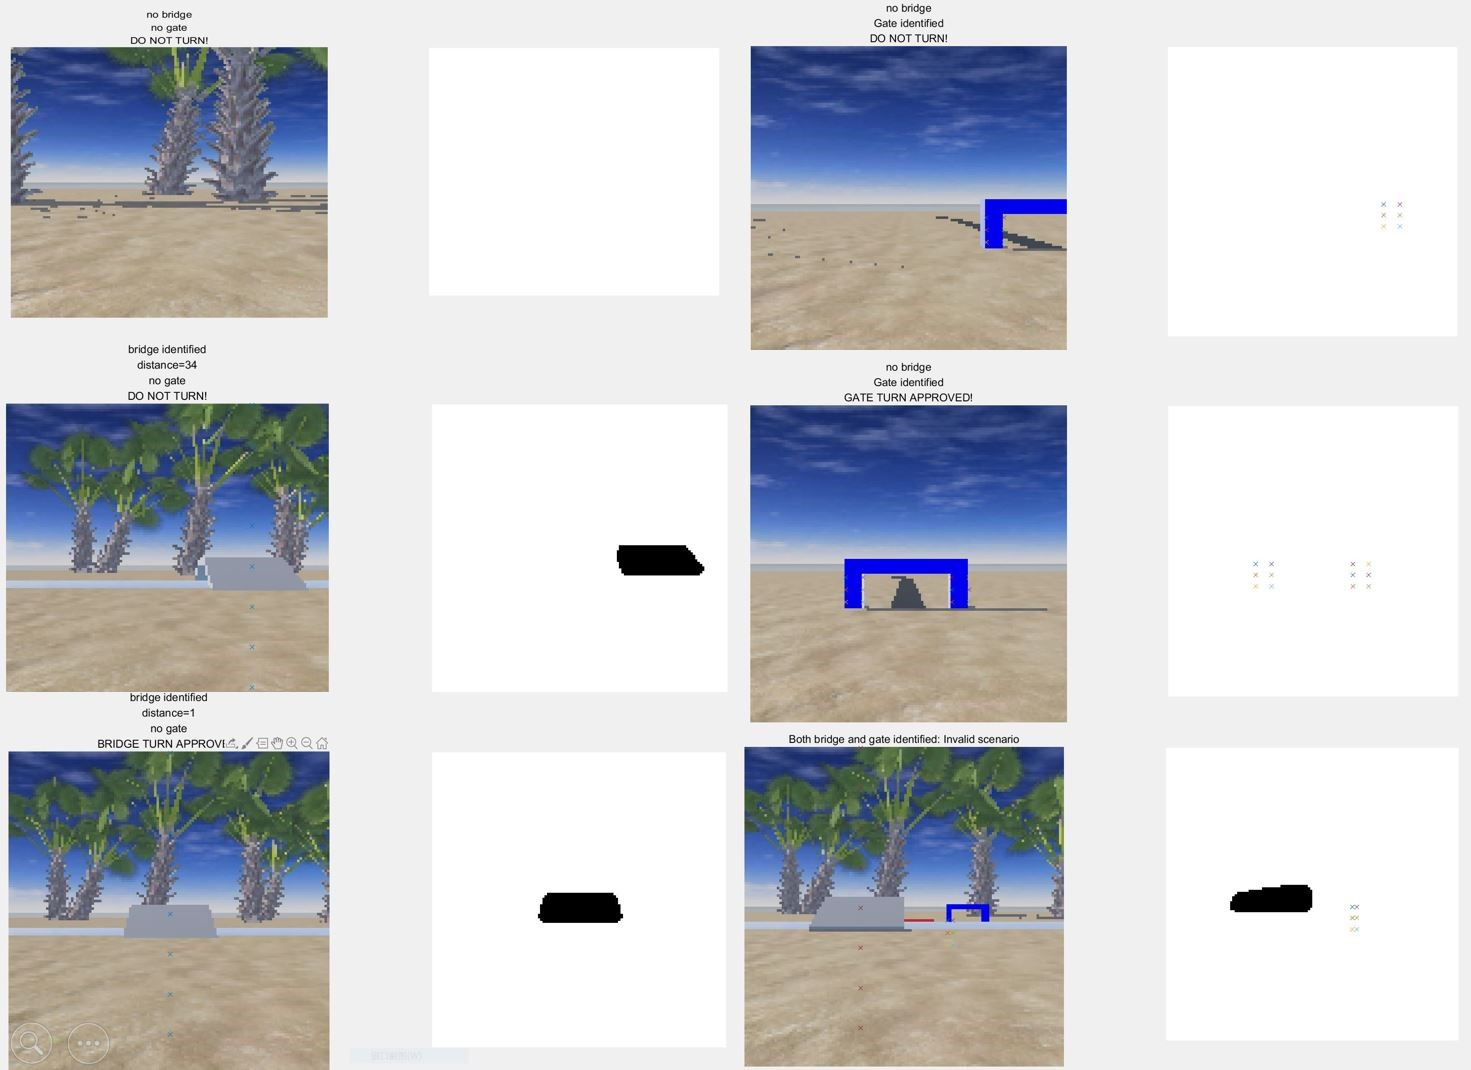
\includegraphics[width=8cm]{implementation/img_wen/object_detection.jpg}
    \caption{The illustration of the bridge detection (left) and the gate detection (right)}
    \label{fig:bridge_and_gate detection}
\end{figure}

In order to give the rover corresponding instruction at the correct location in task 2 to 4, our object detection algorithm involves two parts: object detection and location acquisition.

\begin{enumerate}
    \item \textbf{Object detection}:\\ 
    We detect the objects in tasks 2 to 4, namely the fish tank, the bridge and the gate, by some of their most significant image features, respectively. The fish tank is already detected by the beacon detection algorithm in Section \ref{sec4.2.1}. The bridge is detected by the grayscale feature and the gate is detected by its gradient feature on the edge of its pillar. However, judging whether the object is detected from sole feature of these objects can sometimes be inaccurate. Thus, we further process these features by matrixes computation, including erosion and columns unification, etc. to extract pixels in the image that truly belongs to our target. 
    \item \textbf{Location acquisition}:\\
    We calculate the geometric center of the object according to its extracted features, and compare it with the center of our rover (which is calculated by the camera location) to decide whether the rover is at correct location to execute the next order.
\end{enumerate}

Finally, our rover is able to successfully detect the objects and return corresponding signals so that the Decision Group can give further instructions to control the rover.
%-----------------------------------------------------------------------
\subsection{Sensor Selection \& Implementation}
Author: Haoran HAN, UoG ID: 2357662H\\

In order to accomplish all algorithms described above, we need to choose the right sensors to capture the information from the environment so that the rover could make decisions according to the environment.

At the very beginning of this project, five types of sensor have been tested, including Distance Sensor, GPS, Accelerator, Compass and the Camera. 

The \textbf{Distance Sensor} could provide the distance between the rover and the nearby object. The maximum distance that this sensor could detect and the corresponding precision could be modified in the “LookupTable” property. This sensor is originally designed to detect trees after the rover passing the bridge. The \textbf{GPS} could provide the position of the rover at the coordinate of the whole world. The returned value is the same as the “translation” property of the rover. Moreover, as the name indicates, the \textbf{Accelerator} could return the acceleration of the rover, both the magnitude and the direction in the Cartesian coordinate form. However, as the project developed, team members come up with more brilliant method. In that case, the position, speed, acceleration and the distance between the rover and the environment becomes unnecessary. In that case, even though these three sensors have been tested thoroughly, they are deleted in the final project design.

The \textbf{Compass} will return direction where the x-axis of sensor pointing to. By modifying the x-axis of the Compass to the same as the head of the rover, we could provide the moving direction of the rover in real-time. However, the original returned value is in the Cartesian form which is not easy for the decision group to analysis. In that case, the direction is transformed to the angle that the moving direction deviate from the x-axis and negative z-axis by applying the "arctan" function.

\begin{figure}[htbp]
    \centering
    \subfigure[Picture from Webots GUI]{
    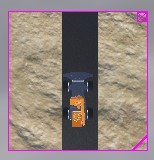
\includegraphics[width=3.85cm]{implementation/img_han/picture_GUI.jpg}
}
    \subfigure[Picture before processing]{
    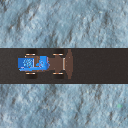
\includegraphics[width=4cm]{implementation/img_han/picture_before_processing.png}
}
    \subfigure[Picture after processing]{
    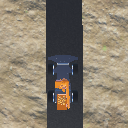
\includegraphics[width=4cm]{implementation/img_han/picture_after_processing.png}
}
    \caption{The comparison among pictures before and after the processing}
    \label{fig:camera}
\end{figure}

The most important sensor in this project is the \textbf{Camera}. The direction that the camera scene towards is the along the negative z-axis and the upper while the upper direction of the camera is along the y-axis. By modifying the “height” and “weight” property, the number of pixels could be changed. However, there exist some problems with the camera: (1) the direction of the picture returned by the python function is not accord with that shown in the GUI; (2) the returned picture is in the RGB form which is not with the BGR required by the opencv package; (3) there is a thin black line (where its RGB channel are all zeros) which could negatively influence the path and object detection algorithm. In that case, the rotation, reshape and crop operation is added after the Camera returning the picture. The comparison among pictures before and after the processing is shown in Figure \ref{fig:camera}. To make it easier to test our path finding algorithm, we define a "capture" function to save the image.

The final design utilizes two Cameras plus a Compass. One Camera towards down directly. This camera is named as “path\_cam”, and it is used for the \textbf{color filtering algorithm} and \textbf{path finding algorithm} developed before. Another camera named as “left\_cam” which towards left is mainly used for the \textbf{bridge detection and gate detection algorithm}. The compass provides the moving direction which will serves as the guidance when there is no path. As illustrate before, we set two direction parameters. This is because when the rover turns to the bridge or the gate, it needs to turn to the negative z-axis while when the rover avoids the tree, it needs to turn to the x-axis. That’s why these to direction is selected. 

\begin{table}[htbp]
\caption{The detailed information of signals processed by the Visual Group\label{tab:details}} 
\begin{tabular}{lcl}
\toprule 
\textbf{Signal Name}     & \textbf{Type} & \textbf{Description}\\ 
\midrule
\tabincell{l}{Direction\_x}   & \tabincell{l}{Float} & \tabincell{l}{Range from -180 to 180. Return the moving direction of the \\
rover that deviates from the x-axis. Left deviation returns \\
negative value, right for positive one}\\
\tabincell{l}{Direction\_-z}   & \tabincell{l}{Float} & \tabincell{l}{Range from -180 to 180. Return the moving direction of the \\
rover that deviates from the negative z-axis. Left deviation \\
returns negative value, right for positive one}\\
\tabincell{l}{Beacon}   & \tabincell{l}{String} & \tabincell{l}{Return “tank detected” when the orange is detected; Return \\
“after bridge” when the green is detected}\\
Path\_Color       & String   & Return the color of the path in Task 5\\
\tabincell{l}{Path\_Direction}   & \tabincell{l}{Float} & \tabincell{l}{Return the moving direction of the rover that deviates from\\
the path. Left deviation returns negative value, right for\\
positive one}\\
Bridge\_Detection & Boolean  & Return “True” when the bridge is detected\\
Gate\_Detection   & Boolean  & Return “True” when the ate is detected\\
\bottomrule
\end{tabular} 
\end{table}

Overall, we explore  a variety of sensors to take advantage of our proposed algorithms and complete the tasks. The final solution is only using two cameras and one compass for the sake of simplicity.
%-----------------------------------------------------------------------
\section{Decision Making\label{sec4.3}}
The Decision Group works as the "brain" of the Mihotel Rover, receiving and processing the signal information from the Visual Group and send commands to the Chassis Group to lead the rover finishing the whole mission. Our work can be divided into two parts, task identification and decision code writing. There are two member in the Decision Group, who are Zijian Wang and Hanpeng Xu. Their work is introduced separated in this section. 
\subsection{Task Identification \& Path Following Decision Making}
Author: Zijian WANG, UoG ID: 2357660W\\

As for the task identification, in order to accomplish the whole process accurately and efficiently, at the beginning of the project, we check our mission and decided to make our initial flow chart. It can help us clear what we need to achieve and what information we can get and use from the project requirement. In the project process, especially when there are several people do the co-operation, the flow chart can significantly increase the readability of the code, help us clear the logic and debug.

The Graphviz really helps us a lot in finishing and improving our logic graph step by step. Comparing with traditional freehand sketching to record our work, the Graphviz has its natural advantages because it takes descriptions of graphs in a simple text language and make diagrams in useful formats. It means that we can easily correct our wrong scheme and add details directly to the flow chart by changing our code. 

\begin{figure}[htbp]
    \centering
    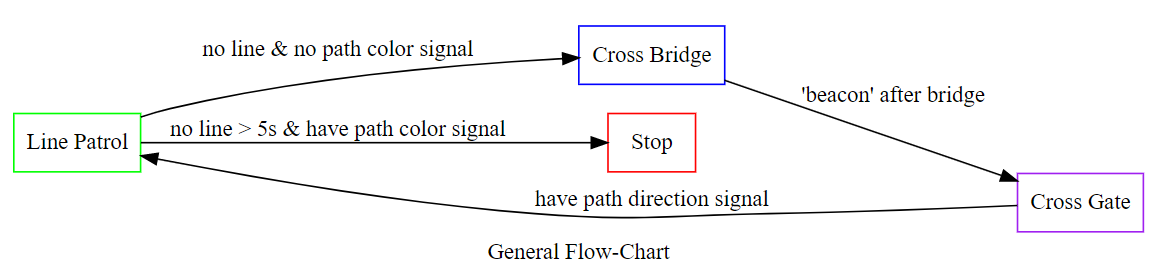
\includegraphics[width=14cm]{implementation/img_zijian/flowchart.png}
    \caption{The general flow chart}
    \label{fig:flowchart}
\end{figure}

As is shown in Figure \ref{fig:flowchart}, the whole process is finished by three states of our rover, line patrol, crossing bridge and crossing gate. The connection relationship and trigger condition can be seen clearly in our GFC. The 3 states include 5 subtasks in the whole process, normal line patrol, feeding, crossing bridge, crossing gate and the color line patrol. Through our merger and simplification, we use the streamlined code and as few as possible states to finish our project. And the transition conditions between each two states were discussed again and again with the Visual Group.

\begin{figure}[htbp]
    \centering
    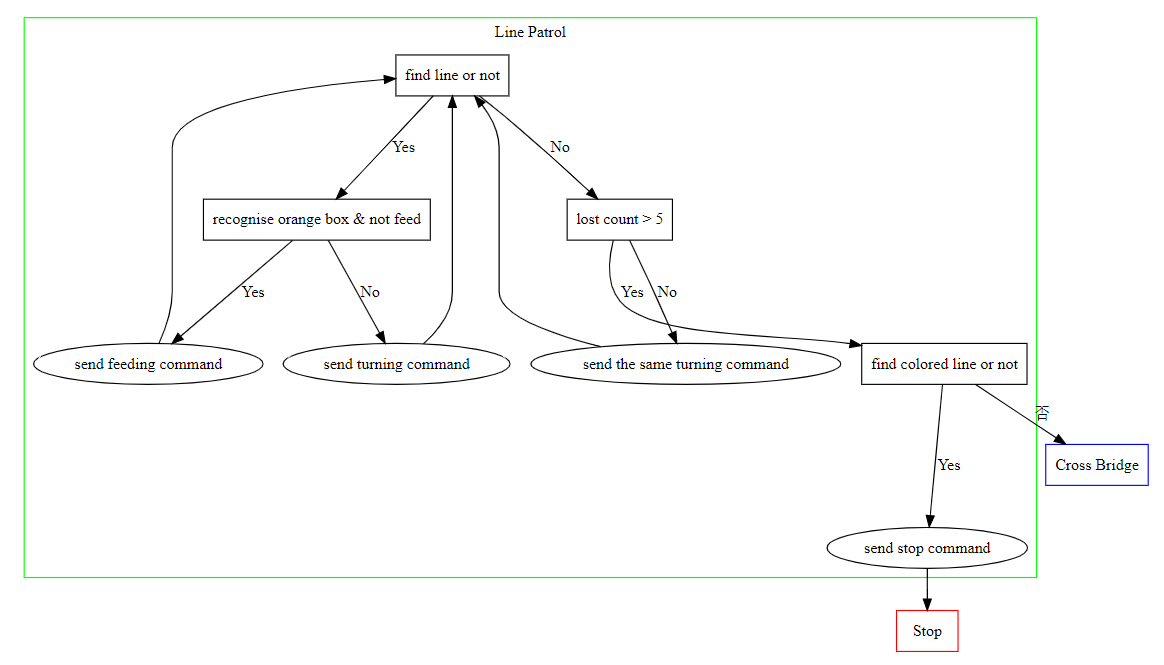
\includegraphics[width=14cm]{implementation/img_zijian/line_patrol.png}
    \caption{The line patrol logic graph}
    \label{fig:line_patrol}
\end{figure}

In the line patrol logic graph shown in Figure \ref{fig:line_patrol}, several important signal judgements can be noticed. We design them as the key nodes to send correct commands to our chassis. “find line or not” is the basic condition for the rover to follow the line direction from the camera image. The orange box signal from visual group and the “no feed” status record work together to guarantee it can execute feed command at orange box for just one time. And the color signal helps us to know whether we have finished our whole process or not. The lost count signal is one of the key designs of our decision group. Even though the color line may be separated at the intersection, the rover can still keep driving ahead until it reaches the real finish position. Because of the tight logic design and detail correction again and again, our rover can deliver the correct command for each signal accurately.

%-----------------------------------------------------------------------
\subsection{Bridge \& Gate Crossing Decision Making}
Author: Hanpeng XU, UoG ID: 2357916X\\

The crossing of the gate and bridge is another focus of our task. In the process of drawing up the flow chart, we overcame many difficulties: (1) How to stop the rover from turning when it came to the bridge; (2) How to prevent the rover from falling on the bridge and make it cross the bridge smoothly. For the first question, after discussing with the vision group, we decided to use the left camera to capture the bridge, so that the camera and the center line of the bridge can be aligned before turning. The second problem was solved by the technical team, who made the rover go wirelessly according to the gyroscope so that it wouldn't fall off the bridge.

\begin{figure}[htbp]
    \centering
    \subfigure[cross bridge]{
    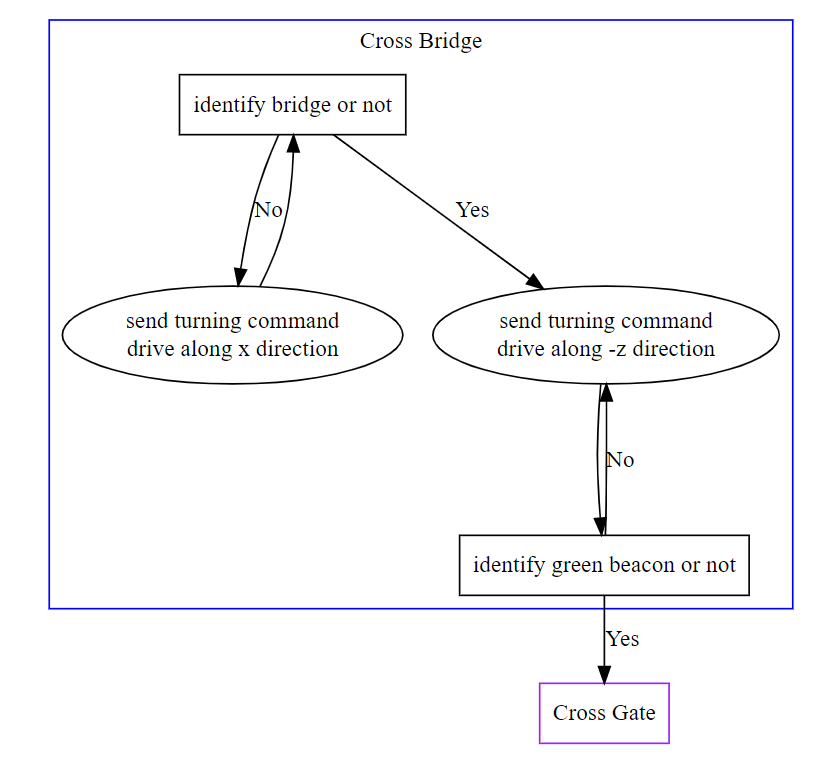
\includegraphics[width=6.3cm]{implementation/img_xu/cross_bridge.png}
    }
    \subfigure[cross gate]{
    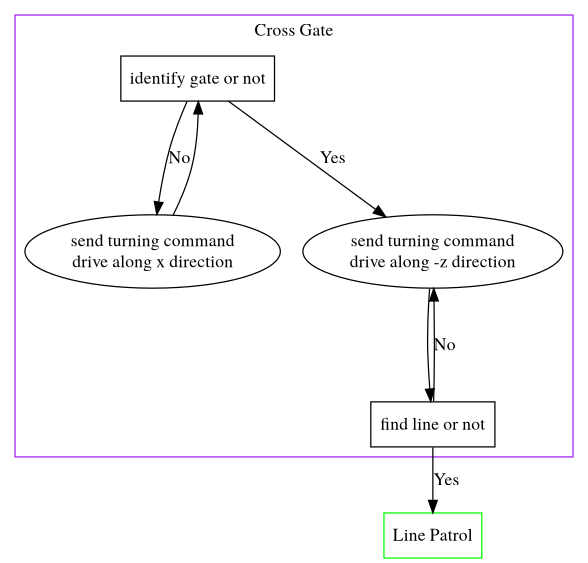
\includegraphics[width=6cm]{implementation/img_xu/cross_gate.png}
    }
    \caption{The flow chart of crossing the bridge and gate}
    \label{fig:cross_bridge_gate}
\end{figure}
After finalizing the final version of the flow chart, the focus of our task shifted to translating the flowchart into Python code. In this process the task, the key to the work is communication. In constant consultation with other technical groups, we make decisions based on the information and conditions that the visual and chassis groups can provide. So, we often have meetings with other technical groups during this period. For example, What code structure is used to execute the command, and what is the overall framework of the code. In addition, we will also go to GitHub above reference others code structure is how to build, and then try to run in the Jupyter Notebook.

\begin{figure}[htbp]
    \centering
    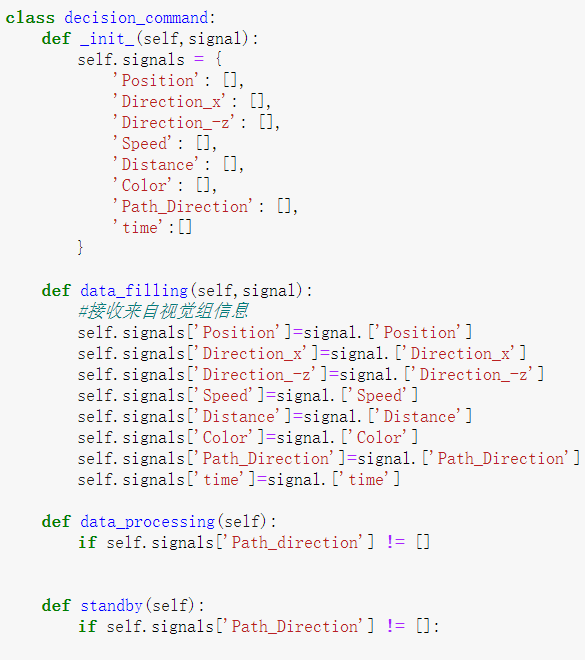
\includegraphics[width=7cm]{implementation/img_xu/decision_code.png}
    \caption{The decision code}
    \label{fig:decision_code}
\end{figure}
%-----------------------------------------------------------------------
\section{Chassis Designing\label{sec4.4}}
The chassis functions as the "body" of our Mihotel Rover. It receives instructions from the Decision Group and control the movement of the rover. There are two member in the Chassis Group. Haotain Wang takes charge of the modeling and importing of the arm and chassis of our rover while Chaofan Shi build the design the control algorithms.

\subsection{Chassis \& Arm Modeling}
Author: Haotian WANG, UoG ID: 2357667W\\

In order to model the rover, the main work of the chassis modeling is to model our design in SolidWorks and transfer it to Webots, and add some necessary node to finish the task. We propose a four-fold modeling process, including chassis selection, coordinate assigning, model simplification and texture assigning.

At the beginning, we planed to assemble a real rover. So we browsed on the e-shop and found several choices. They are shown in Figure \ref{fig:3d_model}. Considering the tasks we have to accomplish, we finally decided to use the four wheel drive chassis(the last one of the following). The chassis had to be stable enough to hold the feeder and cross the bridge. A lower center of mass would be preferred. However, the chassis cannot be too low so that it won't hit the ground when it crosses the bridge. Thus, the other three chastises were abandoned. After we were informed to simulate the task in Webots, we found the 3D model of chosen chassis and proceed the following work. 

\begin{figure}[htbp]
    \centering
    \subfigure[model one]{
    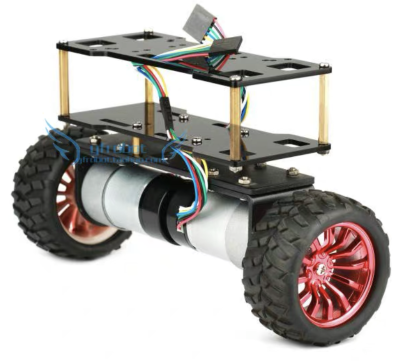
\includegraphics[width=7cm]{implementation/img_haotian/3D_model_1.png}    
    }
    \subfigure[model two]{
    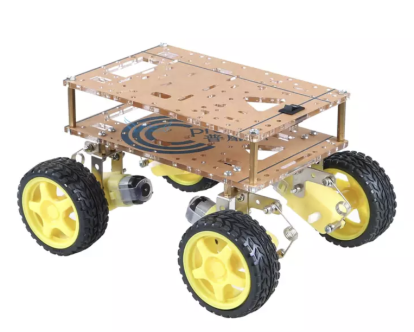
\includegraphics[width=7cm]{implementation/img_haotian/3D_model_2.png}    
    }
    \subfigure[model three]{
    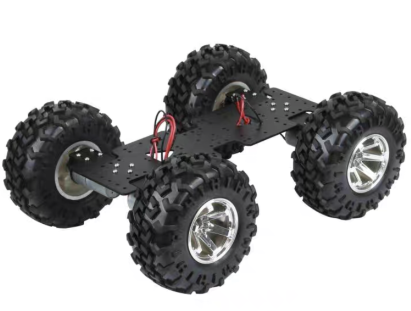
\includegraphics[width=7cm]{implementation/img_haotian/3D_model_3.png}    
    }
    \subfigure[model four]{
    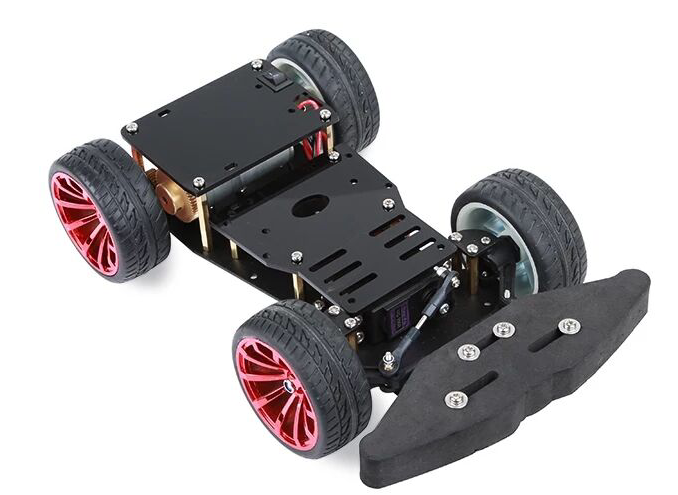
\includegraphics[width=7cm]{implementation/img_haotian/3D_model_4.png}
    }
    \caption{The 3D models on e-shops}
    \label{fig:3d_model}
\end{figure}

Before we import the chassis into the simulated world, we had to set the coordinates of each component, especially for the wheels. If the axes of the wheels were not properly assigned. Wheels won't rotate as expected. We shows the difference between wrongly and properly assigning coordinates to the wheel in Figure \ref{fig:coordinates}.

\begin{figure}[htbp]
    \centering
    \subfigure[not assigned to the wheel]{
    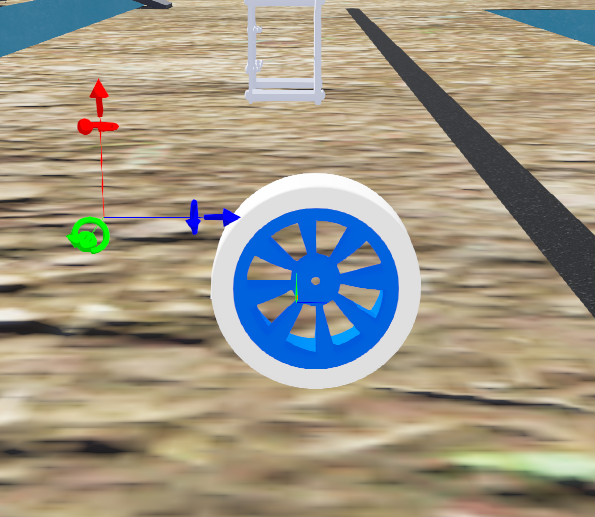
\includegraphics[width=5.73cm]{implementation/img_haotian/coordinates_of_wheels_1.png}    
    }
    \subfigure[properly assigned to the wheel]{
    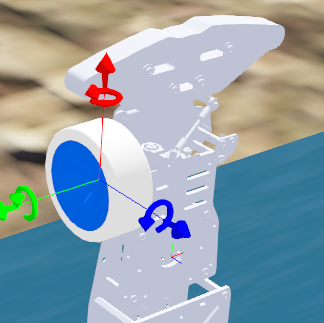
\includegraphics[width=5cm]{implementation/img_haotian/coordinates_of_wheels_2.png}    
    }
    \caption{Coordinates assigned to the chassis}
    \label{fig:coordinates}
\end{figure}

The original model contained too much unnecessary details which affect the performance of the simulation. Therefore, we had to delete some less important components while keeping the its appearance unchanged. Simplification is accomplished using SolidWorks. The simplified model is shown in Figure \ref{fig:simplified_model}. The simplified model could run smoothly in the simulation world.

\begin{figure}[htbp]
    \centering
    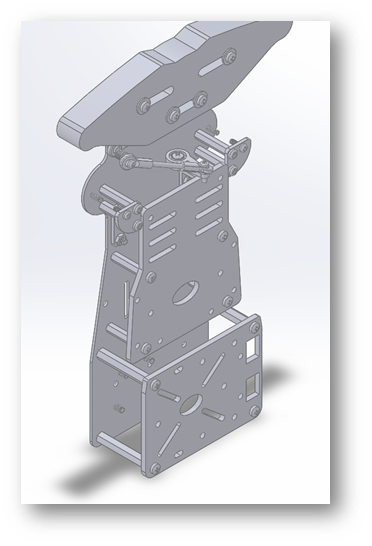
\includegraphics[width=7cm]{implementation/img_haotian/simplified_model.png}
    \caption{The simplified model}
    \label{fig:simplified_model}
\end{figure}


The imported models are unpainted at first. In order to make the rover looks more fancy, we set an iron material to its body and  rubber to its wheels.

\begin{figure}
    \centering
    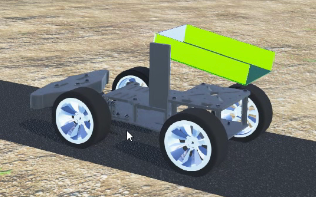
\includegraphics[width=6cm]{implementation/img_haotian/texture_assigning.png}
    \caption{The model with texture assigned}
    \label{fig:texture}
\end{figure}


The final specifications of the chassis are listed in Table \ref{tab:final_specifications}. The density of the chassis and feeder is set as different materials. The feeder is much lighter than the chassis. this design is for maintaining the mass center of the rover at its geometry center, so the rover can make turns as expected.
\begin{figure}[htbp]
    \centering
    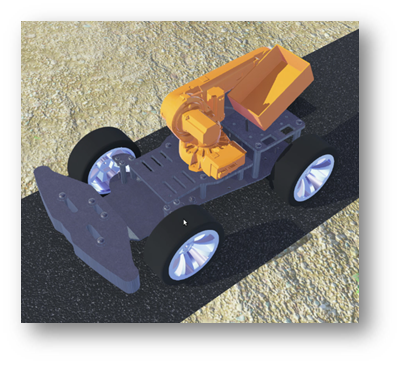
\includegraphics[width=6cm]{implementation/img_haotian/final_design.png}
    \caption{The final design}
    \label{fig:final_design}
\end{figure}

\begin{table}[htbp]
    \centering
    \begin{tabular}{llll}
    \toprule
    \multicolumn{1}{l}{}    & \textbf{Item}                 & \textbf{Specification}                                        & \textbf{Note}               \\
    \midrule
\multirow{2}{*}{Body}   & size                 & 0.15 m $\times$ 0.23 m $\times$ 0.05 m               & width $\times$ length $\times$ height             \\
                        & density              & 7.85 $\times 10^3$ kg/$m^3$                          & density of metal                                  \\
\multirow{6}{*}{Wheel} & radius               & 0.033 m                                              &                                                   \\
                        & max velocity         & 100 rad/s                                            & move forward when velocity is negative          \\
                        & max torque           & 100 N $\cdot$ m                                       &                                                   \\
                        & front track          & 0.12 m                                               & velocity distance from center is 0.068 m          \\
                        & rear track           & 0.12 m                                               & velocity distance from center is 0.07 m           \\
                        & motor control method & velocity control                                     & PID is not used in velocity control               \\
\multirow{5}{*}{Arm}    & density              & 0.8 $\times 10^3$  kg/$m^3$                          &                                                   \\
                        & arm length           & 0.035 m                                              &                                                   \\
                        & max velocity         & 20 rad/s                                             &                                                   \\
                        & max torque           & 100 N $\cdot$ m                                       &                                                   \\
                        & holder size          & 0.04 m $\times$ 0.066 m $\times$ 0.024 m              & width $\times$ length $\times$ height             \\            
    \bottomrule
    \end{tabular}
    \caption{The final specifications of the chassis}
    \label{tab:final_specifications}
\end{table}
%-----------------------------------------------------------------------
\subsection{Chassis \& Arm PID Control}
Author: Chaofan SHI, UoG ID: 2357686S\\

The chassis controlling of the Chassis Group focuses on solving the controlling problems and writing the chassis controlling algorithms. We break down this into three parts: (1) adjust the centre of mass of the rover; (2) design the arm control algorithm; (3) adjust the PID control of the chassis.

In order to control the rover, the first thing needed to be solved is the rotation problem. When we want it rotate in place, the centre of mass will move around the centre. If the speed is fast, the rover will even fall apart. So, we tried some methods to solve this problem. We firstly tried to adjust the mass of four wheels and the mass of  the chassis. Then we found the rover will oscillate greatly, even separate the rover if we increase the mass of the wheel greater than the chassis. Secondly, we tried to adjust the relative position of four wheels to make it a square, and it proves to be useless. Thirdly, we compare the car with 4-Wheels robot in the tutorial\cite{tutorial_2}, and we realized it may only related with the centre of mass. After we finally found that the reason is caused by the centre of mass,  we moved the bounding object of the rover and adjust the position to solve the problem. The centre of mass of our rover is illustrated by Figure \ref{fig:centre_of_mass}.

\begin{figure}[htbp]
    \centering
    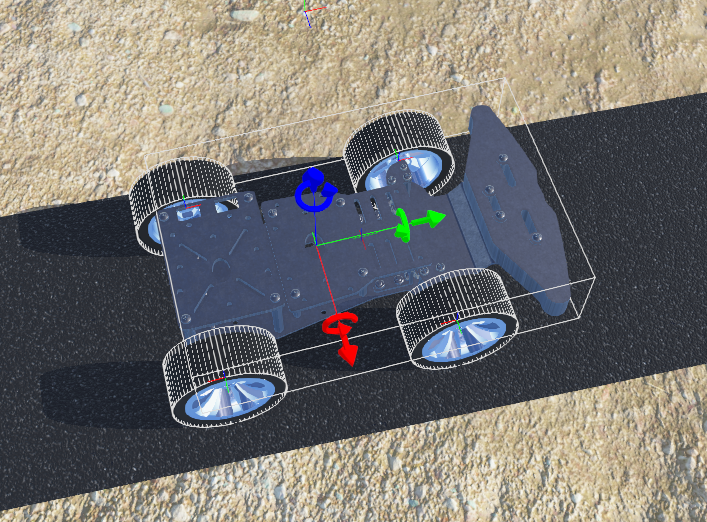
\includegraphics[width=6cm]{implementation/img_shi/centre_of_mass.png}
    \caption{The centre of mass of the rover}
    \label{fig:centre_of_mass}
\end{figure}

Next, we need to control the arm to deliver the fish food, and we want to release the fish food both safely and elegantly. In fact, we choose to set its position directly at first, However, in the former version, we choose to throw the food without stop, so we have to set speed and us position limitation, because we can not precisely control the number of loops during a period. Using time delay and the speed control also contains some problems, it can not precisely control the position of the arm, so sometimes the position would be a little different.

\begin{figure}[htbp]
    \centering
    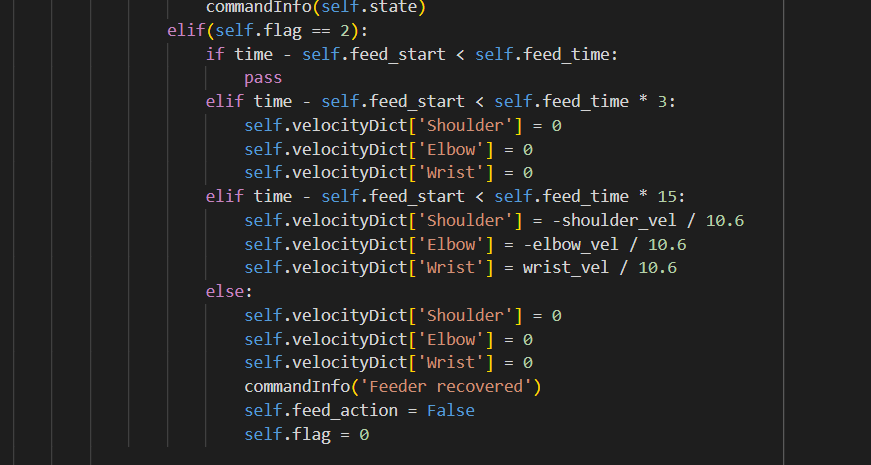
\includegraphics[width=10cm]{implementation/img_shi/arm_control.png}
    \caption{arm control algorithm}
    \label{fig:arm_control}
\end{figure}

The last control algorithm is about the chassis. Our target is to move the car as fast as possible and finish the whole project in a rapid and steady fashion. Since the chassis receives the angle, which can be further converted into speed, the only thing for the chassis control is to write a PID program to transfer angle to speed, which is shown in Figure \ref{fig:PID_control}.

\begin{figure}[htbp]
    \centering
    \subfigure[]{
    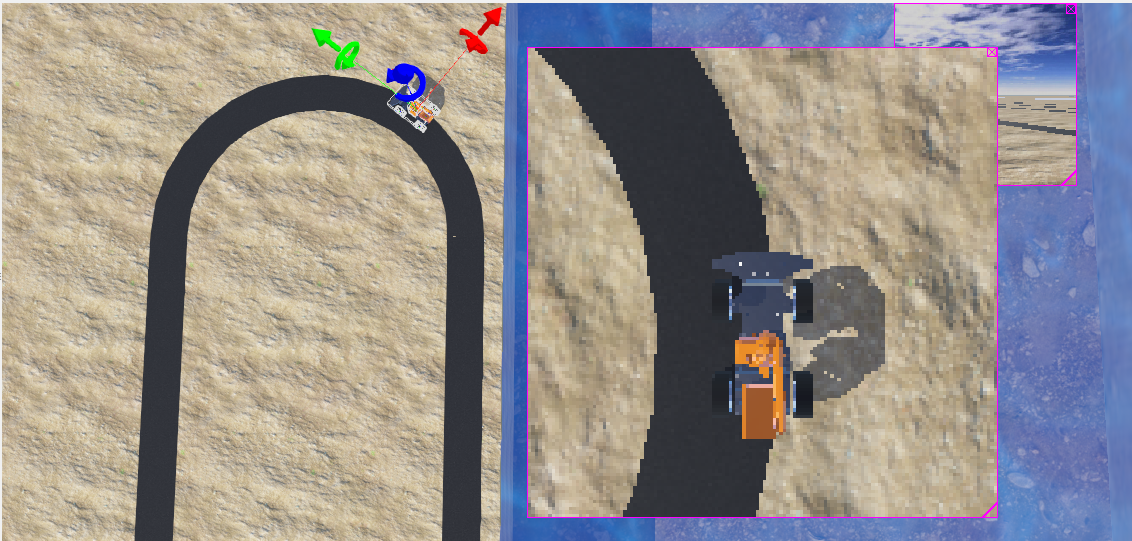
\includegraphics[width=6.5cm]{implementation/img_shi/PID_control_1.png}
    }
    \subfigure[]{
    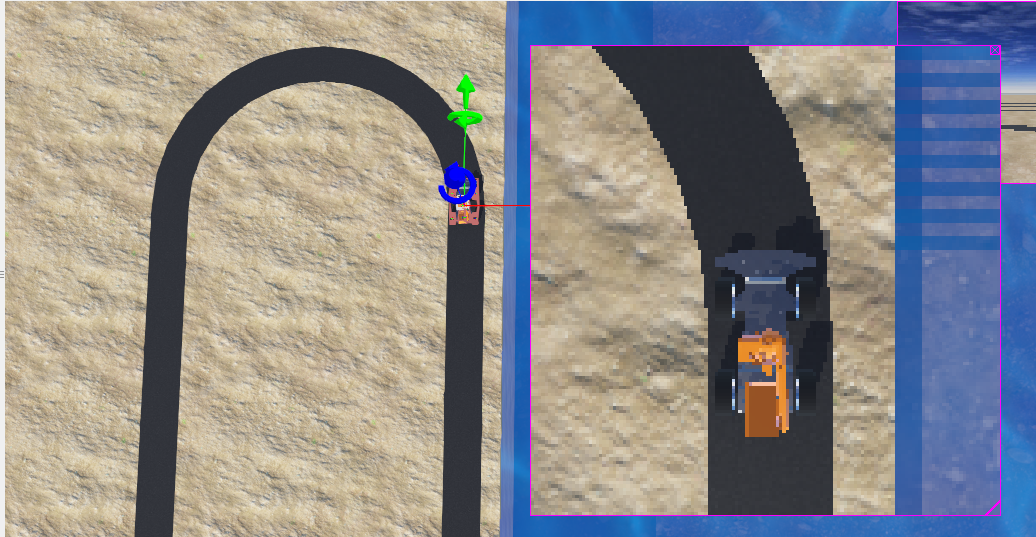
\includegraphics[width=6cm]{implementation/img_shi/PID_control_2.png}
    }
    \caption{The PID control of chassis}
    \label{fig:PID_control}
\end{figure}

Our controlling method is writing a forward speed and adding the steering speed by the angle we received from decision group. At first, we want to use the PID control method, because it can both reduce the overshoot in curve and make the oscillation better in the straight road. However, it dose not work because the command the rover received has a delay compared the simulation time, so the derivative and integral part will make the performance worse.  Then we found some frames have lost because the sensors wound cost a lot of times to refreshing and processing its data. Therefore, we add the limitation of the system to solve the former controlling problem.

\begin{figure}[htbp]
    \centering
    \subfigure[with frame loss]{
    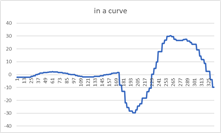
\includegraphics[width=6cm]{implementation/img_shi/with_frame_loss.png}
    }
    \subfigure[without frame loss]{
    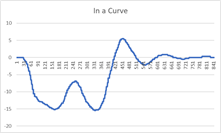
\includegraphics[width=6cm]{implementation/img_shi/without_frame_loss.png}
    }
    \caption{The PID control with and without frame loss}
    \label{fig:frame_loss}
\end{figure}

During experiments, the frame has 3 or more loss in each second, thus causing the rover to oscillate greatly. Hence, we have to add the limitation although we can get a faster simulation speed without the limitation. After we add the limitation, we can observe that the angle reduced from above 30 degree to about 15 degree, and the setting time reduced a lot. the rover perform much better. 

At last we reduced the speed of the rover and increased the proportional control of it. As a result, we effectively prevent the overshoot problem around the corner.
%-----------------------------------------------------------------------
\section{System Controlling\label{sec4.5}}
The system controlling part is in the charge of our tech leader, Zhuheng Song. 
\subsection{Multiprocessing \& Code Refactoring}
Author: Zhuheng SONG, UoG ID: 2357651S\\

\begin{figure}[htbp]
    \centering
    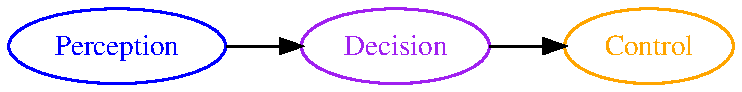
\includegraphics[width=14cm]{implementation/img_song/regular_development.pdf}
    \caption{The regular development process}
    \label{fig:regular_development}
\end{figure}

There is no doubt that a whole control process goes like this:
\begin{enumerate}
    \item Abstract data from sensors into signals to show state of the rover
    \item Make decision of following behavior depending on current state
    \item control the rover to do the required behavior
\end{enumerate}

Since here we do not have very complex situations to make decisions and we do not have to very complex tasks to do, it is obvious that \textbf{each stage takes different amount of time}. I suppose \textbf{Perception} takes a lot time, while time cost by \textbf{Decision} stage may be really short that we could even ignore it. In addition, \textbf{Control} stage actually need an \textbf{separate}, \textbf{high frequency} loop to keep high precision control of the rover.

Therefore, we need three separate loops:
\begin{itemize}
    \item A perception loop keeps processing sensors data and transmit signals to decision loop. It should send out signals every time a signal is updated, but not send once when all signals are updated. In this way, we could always do decisions with the latest signals.
    \item A decision loop keeps sending commands to control loop depending on signals received from perception loop.
    \item A control loop keeps controlling the rover to act like what the decision loop asks to do, for example applying a PID control on velocity of four wheels.
\end{itemize}

Then we found two normal ways to allow three separate loops in one program: (1) multi-processing; (2) multi-threading

After some research we found that: If your program is a \textbf{CPU intensive} application, multi-processing is recommended, While multi-threading is more suitable for \textbf{I/O intensive} applications.

\begin{itemize}
    \item A CPU intensive application is: for example, which has lots of loops or calculating steps.
    \item A I/O intensive application is: for example, mainly deal with files, or a web crawler.
\end{itemize}

Since multi-threading is running concurrently, most implements use a counter to decide whether switch to another thread. Therefore a CPU intensive application could reaches the counter threshold very soon, and need to compete for time to execute again.

On the other hand, for I/O intensive applications which have lots of situations where has to wait for \textbf{external} events, multi-threading could save a lot of resource, as for these situations, we could switch to another thread.

\begin{figure}[htbp]
    \centering
    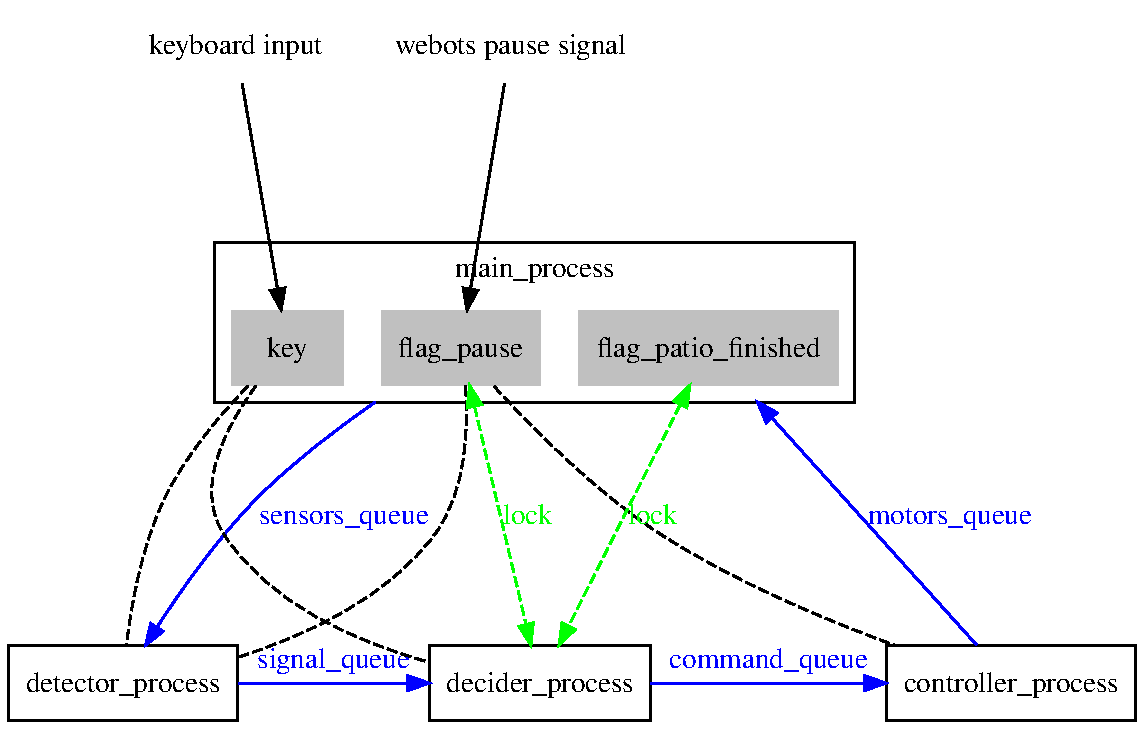
\includegraphics[width=12cm]{implementation/img_song/system.pdf}
    \caption{The final structure of our system}
    \label{fig:system}
\end{figure}

Given this, we decide to design a \textbf{multiprocessing} system. After lots of experiments, the system is developed to allow multiprocessing even in Webots, cross-platform and with high performance. The final structure of our system is shown in Figure \ref{fig:system}.

The \textbf{detector process} will process sensors data and send all signals to the \textbf{decider process }every time a signal is updated, then the \textbf{decider process} will send command to the \textbf{controller process}, where the command is parsed into a dictionary of motors velocity. In addition, no matter a command is sent to \textbf{controller process} or not, it will send the motors velocity dictionary to the main process once every 5 ms. And before receiving the motors velocity dictionary, the main process will be blocked for 20ms, leave time for the three processes to do the work. Therefore, the simulation speed is now $\frac{32}{30+a+b}$, almost the best we could do, since we could not reduce a and b from the code. According to my test, value of $a+b$ could vary \textbf{from 10ms to 70ms}.

Figure \ref{fig:final_control_loop} shows delays in the cycle.

\begin{figure}[htbp]
    \centering
    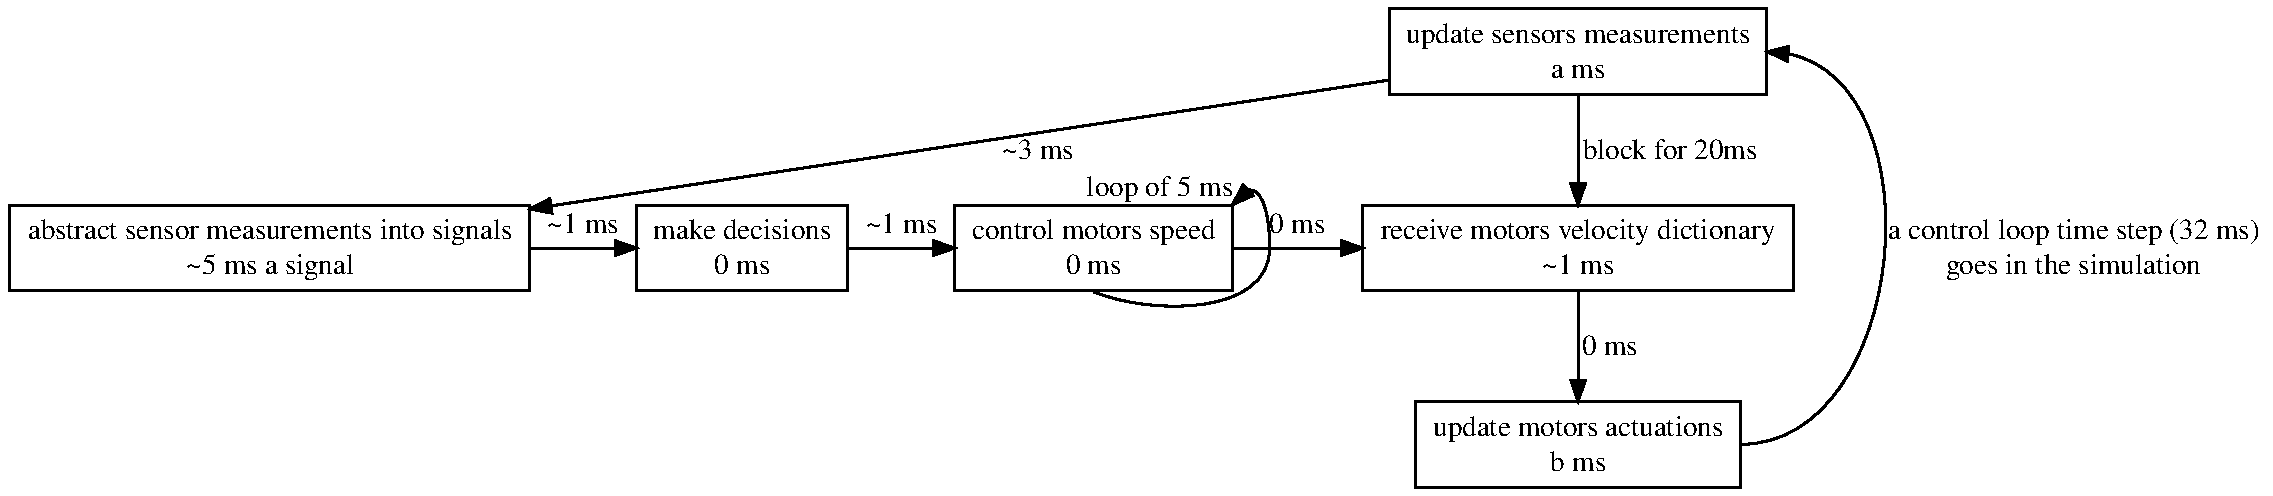
\includegraphics[width=14cm]{implementation/img_song/final_control_loop.pdf}
    \caption{The final control loop}
    \label{fig:final_control_loop}
\end{figure}

To prove the system works as expected, every step and the time it cost is logged, to show the exact time and order. It can be seen from the output shown in Figure \ref{fig:system_output} that there is at most delay of one frame between the simulation and motors velocity, which means in the simulation the motors velocity has a delay of at most 32ms. This is what expected and it is acceptable for this program.

\begin{figure}[htbp]
    \centering
    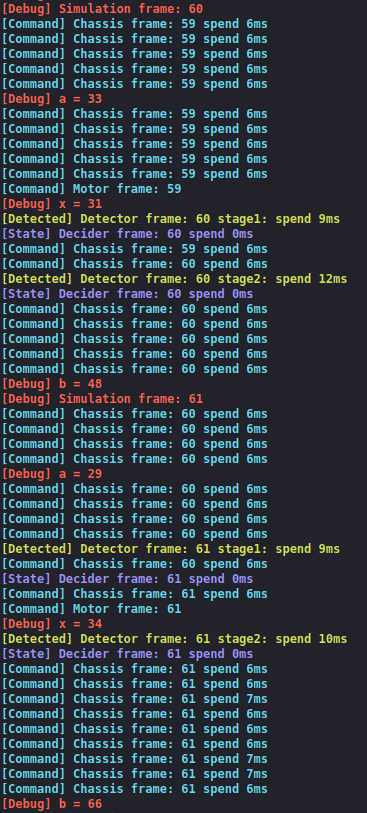
\includegraphics[width=5.5cm]{implementation/img_song/output.png}
    \caption{The system output}
    \label{fig:system_output}
\end{figure}